\documentclass[final,creativeai]{article}
\usepackage{neurips_2025}

\usepackage[utf8]{inputenc}
\usepackage[T1]{fontenc}
\usepackage{hyperref}
\usepackage{url}
\usepackage{booktabs}
\usepackage{amsfonts}
\usepackage{amsmath}
\usepackage{nicefrac}
\usepackage{microtype}
\usepackage{xcolor}
\usepackage{graphicx}
\usepackage[safe]{tipa}  % Lakota eng glyph (ŋ) via \textipa{N}; safe = keep math \!,\; etc.
\usepackage{placeins}    % \FloatBarrier keeps each section's figures within it

% Figures live in paper/v2/figures/ ; this .tex lives in paper/v2/.
\graphicspath{{figures/}{../original/}}

% Citation keys used below that are NOT in the original references.bib are
% provided in references_v2_additions.bib (merge it into references.bib):
%   ethayarajh_contextual_2019, mu_allbutthetop_2018,
%   lewis_indigenous_2020, carroll_care_2020, kukutai_indigenous_2016

\title{Meaning as Relational Rewiring:\\Quantifying Contextual Distortion of Latent Semantics\\in Visual Symbolic Systems}

\author{%
  Antoine Bellemare-Pepin \\
  Department of Psychology \\
  Université de Montréal \\
  Montreal, QC, Canada \\
  \texttt{antoine.bellemare9@gmail.com} \\
  \And
  Suzanne Kite \\
  Wihanble S'a Center \\
  Bard College \\
  Annandale-on-Hudson, NY, USA \\
  \texttt{skite@bard.edu} \\
}

\begin{document}

\maketitle

\begin{abstract}
Visual symbolic systems embody ambiguity, polysemy, and context-dependent meaning: qualities that static language-model embeddings flatten into averaged points. The Lakota Shape Kit, a traditional storytelling tool, exemplifies this richness: each symbol juxtaposes many concurrent readings whose prominence shifts with narrative context. Working from Lakota relational epistemology (\emph{Mitákuye Oyás'i\textipa{N}}, the principle that nothing exists in isolation and that meaning is a thing's position in a living web of relations), we develop a framework that represents each symbol as a context-weighted distribution over semantic descriptors and then asks not merely \emph{which} descriptors a context foregrounds, but \emph{how a context distorts the relational geometry among them}. Our central instrument is the $\Delta$ coupling matrix, the signed change in the pairwise inner-product (Gram) structure of a curated lexicon under a context-shift operator. $\Delta$ localizes contextualization to the lexical relations that strengthen or weaken, providing a grounded, interpretable readout of how narrative framing rewires a symbolic field. We characterize this readout honestly (its dominant component is a first-order, relevance-gated reweighting of the encoder's own contextualization, re-expressed in the community-curated coordinate system) and demonstrate it across several settings: reading a narrative as a trajectory through coupling space, using the distortion profile's margin as an intrinsic uncertainty signal, recovering content-bearing context similarity once a single activation-magnitude artifact is removed, and, because the readout is modality-agnostic, probing the field's ambiguity with sound as well as text. Demonstrated with Lakota symbols and developed in collaboration with a knowledge holder under the Abundant Intelligences program, the framework advances context-sensitive meaning modeling for computational linguistics, cross-cultural knowledge representation, and creative AI.
\end{abstract}

\section{The Lakota Shape Kit}
Language can be understood fundamentally as a relational web, where each word derives its meaning through differences and positional relationships with all other elements in a linguistic system \cite{stawarska_saussures_2020, wood_derrida_1988}. Words seldom possess static meanings; rather, their interpretations shift dynamically according to context, usage, and narrative positioning. This inherent polysemy and context-dependence is particularly pronounced in visual symbolic languages, systems where symbols encapsulate broad, multilayered semantic fields \citep{saint-martin_semiotics_1990}.

The Lakota Shape Kit \cite{wing_learning_2016} exemplifies a visual symbolic system characterized by high degrees of polysemy, interpretive openness, and nonlinear combinatoriality. Traditionally, it provides a nuanced framework for narrating dreams \citep{kite_hel_2023}, inherently designed to preserve and explore multiple concurrent meanings and storylines. Each Lakota symbol, such as the dragonfly or the house, can evoke diverse and sometimes divergent meanings depending on its cultural and situational context, with the relative prominence of each meaning shifting fluidly according to the narrative surroundings.

This work is grounded in Lakota relational epistemology, expressed in the principle \emph{Mitákuye Oyás'i\textipa{N}}, ``all my relations.'' Meaning, in this view, is not a property an object carries in isolation but the position it occupies in a living web of relations among descriptors, contexts, and interpreters. We take this not as decoration on a computational method but as the method's motivation: it tells us \emph{what to look at}. If meaning is constituted by relations, then the right object of study under context is not the displacement of a symbol's vector but the reconfiguration of the relations among its facets. The framework below is a formal expression of that commitment, developed in collaboration with a Lakota knowledge holder within the Abundant Intelligences program, which fosters AI systems built \emph{from} Indigenous knowledge systems rather than merely applied to them \citep{lewis_indigenous_2020}.

\begin{figure}[tbp]
    \centering
    \IfFileExists{figures/fig_symbols.png}{%
      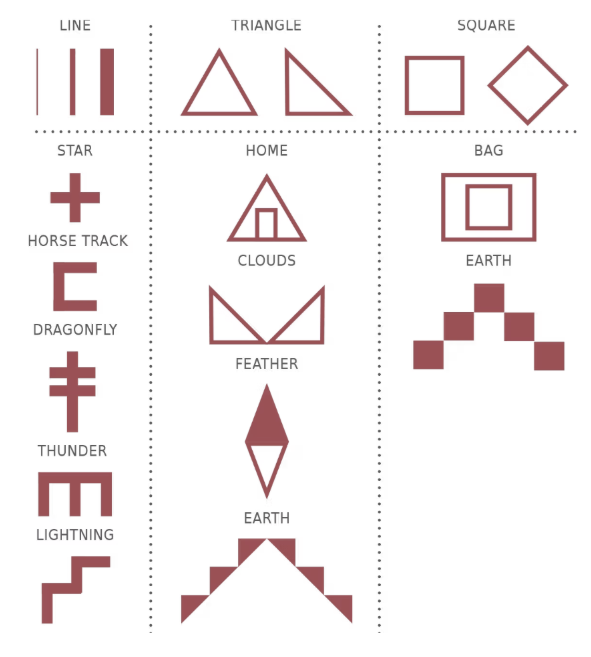
\includegraphics[width=0.4\linewidth]{fig_symbols.png}}{%
      \fbox{\parbox{0.4\linewidth}{\centering\vspace{2.5em} \texttt{fig\_symbols.png}\\ (Lakota Shape Kit plate, drop asset into \texttt{figures/}) \vspace{2.5em}}}}
    \caption{Lakota Shape Kit, a visual storytelling tool rooted in Lakota traditions (from \citep{wing_learning_2016}).}
    \label{fig:lakota_symbols}
\end{figure}

Modern language embeddings are, in fact, remarkably good at \emph{encoding} ambiguity: a trained model packs many senses of a word into a single vector, and contextualized encoders adjust that vector fluidly as the surrounding text changes \cite{haber_polysemyevidence_2024, loureiro_analysis_2021}. The difficulty is not that models cannot represent polysemy, but that this latent ambiguity is neither \emph{legible} nor \emph{relational}. The senses are entangled in an opaque coordinate system rather than organized by the categories of a particular symbolic tradition; meanings underrepresented in training data may be faint or absent (a limitation of data more than of architecture); and, most importantly for a relational epistemology, the encoder exposes the contextualized \emph{vector} of a symbol but not how a context reshapes the web of \emph{relations} among a curated field's facets, which is the level at which meaning here actually lives \cite{ferrari_identification_2018}. The gap, then, is a gap in \emph{instruments}: we lack ways to read how a model internally represents, and contextually reshapes, a community-curated symbolic system.

This paper addresses that gap. Large models already shift a symbol's meaning fluidly with context (this is, in effect, what their attention layers do), but that internal machinery is rarely made inspectable at the level of a \emph{designed} symbolic field. We therefore treat a curated lexicon as a controlled probe into a language model's latent space: each symbol is represented as a distribution over textual descriptors, and, our central contribution, we measure the signed change in the pairwise coupling among those descriptors under context, turning the model's internal reconfiguration into a legible, per-relation readout. We call this \textbf{quantifying how context distorts the latent semantic geometry} of the field.

Our contribution is fourfold: (1) we cast a community-curated symbolic system as a controlled probe into a language model's latent space, making its internal, context-dependent representation of that system inspectable rather than treating context-sensitivity as a black box; (2) we introduce the $\Delta$ coupling matrix, a structural probe that decomposes a context's effect into the lexical relations it strengthens or weakens, and characterize honestly what it does and does not recover; (3) we demonstrate the readout across narrative, uncertainty, and similarity settings, and show it is modality-agnostic: sound probes the field's ambiguity as well as text does; and (4) we situate the work as Abundant Intelligences scholarship, developed with and accountable to an Indigenous knowledge system. Ultimately this research aims to inform AI methodologies developed in active collaboration with Indigenous research projects and grounded in their knowledge systems.

\section{The Inherent Ambiguity of Meaning}
Ambiguity occurs when a signal supports multiple valid interpretations even when well-formed. In language, polysemy (where a single form is linked to multiple related senses) is increasingly regarded as the norm rather than the exception. Empirical and theoretical work shows that ambiguity is not a flaw to be eliminated but a structural feature that supports communicative efficiency \citep{piantadosi_communicative_2012, hermalin_efficient_2019}. On this view, ambiguity is a natural consequence of the pressure to communicate efficiently about a vast and complex world with a finite, reusable set of forms: a compact vocabulary can only cover an open-ended space of meanings if forms are allowed to carry more than one sense, with context doing the work of disambiguation. Network analyses of language are consistent with this, treating ambiguity as a resource that increases expressive power while minimizing effort \citep{sole_ambiguity_2015}.

Information-theoretic accounts further show that all efficient communication systems will be ambiguous if context carries information about meaning \citep{piantadosi_communicative_2012}. Ambiguity enables the reuse of compact, efficient linguistic units, with context selecting the intended interpretation. Visual symbolic systems display similar properties \citep{cohn_visual_2013}: symbols in pictorial narratives or ideographic languages follow conventional compositional rules yet remain underspecified, with meaning resolved through surrounding context. The same visual form can activate distinct interpretations depending on its narrative, situational, and cultural embedding.

These literatures are \emph{resonant} with the relational view we adopt rather than its source. From a semiotic perspective, meaning is triadic: a sign links to its object through the interpretant, the situated act of interpretation \citep{kilstrup_naturalizing_2015, smythe_formal_1998, innis_semiotics_1985}; context stabilizes one among many possible readings. Saussure's relational language and Peirce's triadic sign converge, from a Western direction, on a claim the Lakota tradition states directly: a thing's meaning is its place among relations. We engage these parallels where they converge, and treat the Lakota Shape Kit as the source of theory rather than a case study to which an external theory is applied.

\section{Context-Conditioned Symbol Embeddings}
Building on this notion of ambiguity, we operationalize meaning as a dynamic, context-sensitive process. Instead of a static vector, each symbol is defined by a set of textual descriptors spanning its possible interpretations (e.g., ``flight,'' ``balance,'' ``fertility'' for the dragonfly). Each descriptor is embedded with a state-of-the-art language model (Qwen3-Embedding-0.6B \citep{qwen3_embedding_2025}), giving a row-normalized descriptor matrix $D \in \mathbb{R}^{n \times d}$ for the field. This section characterizes the field \emph{at rest} and introduces the point-level view of contextualization: which descriptors a context foregrounds. Section~\ref{sec:delta} then lifts this to the relational level.

\subsection{The symbolic field at rest}
Inspired by prior work on semantic-network analysis and distributional semantics \citep{steyvers_large-scale_2005, mikolov_efficient_2013, arora_simple_2017}, we quantify the structure of the meaning space with three complementary metrics: \emph{dispersion}, the average dissimilarity among a symbol's descriptor embeddings (spread of its facets); \emph{leakage}, the proportion of each descriptor's nearest neighbors belonging to other symbols (cross-symbol overlap); and \emph{inter-symbolic entropy}, the average Shannon entropy of the softmax-normalized similarities between each descriptor and all symbol centroids (how evenly relevance can be distributed across interpretations). Together these distinguish symbols whose ambiguity is internal (dispersion) from those whose ambiguity arises from external overlap (leakage) or context-sensitive spread of relevance (entropy). Figure~\ref{fig:umap_metrics} illustrates this structure.

\begin{figure}[tbp]
    \centering
    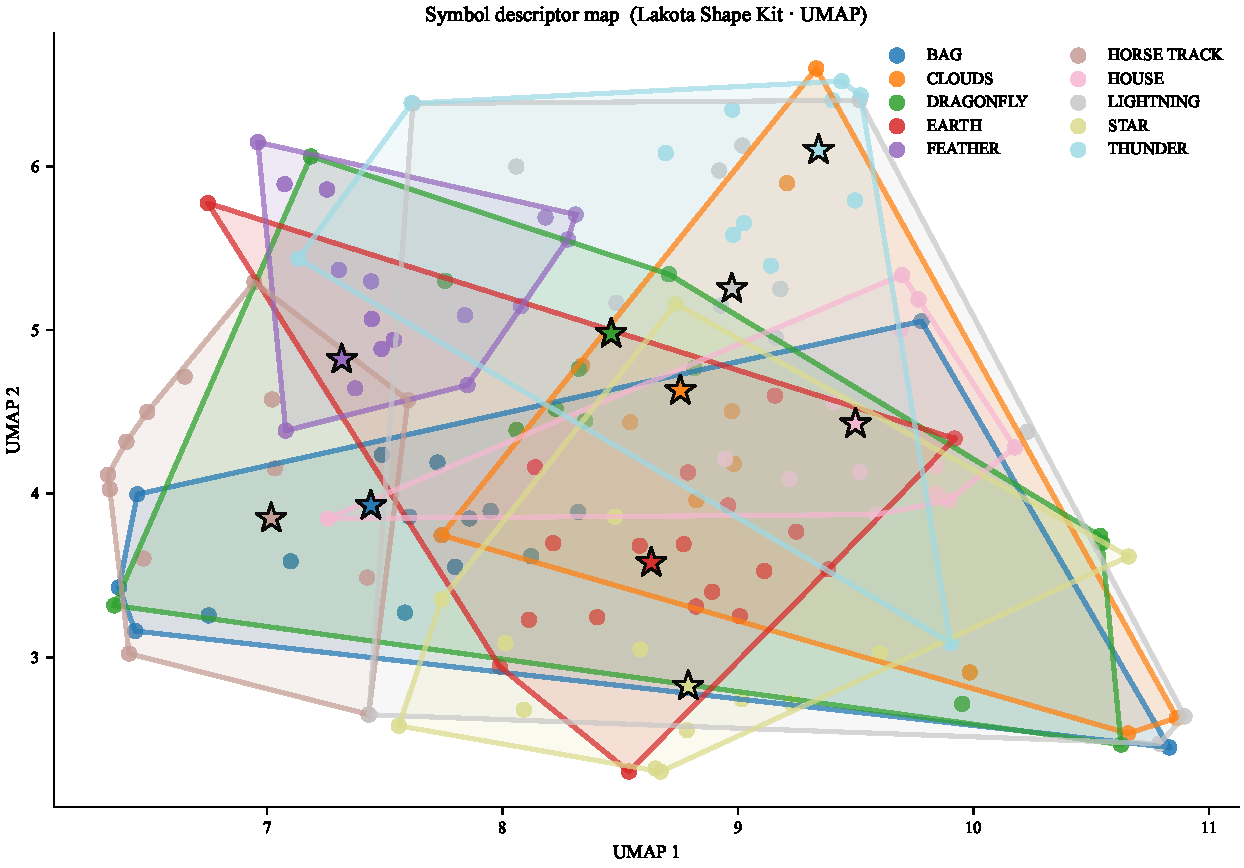
\includegraphics[width=0.9\linewidth]{fig_v1_umap}
    \caption{Symbol--descriptor semantic map with ambiguity metrics. A UMAP projection \citep{mcinnes_umap_2018} shows all symbol descriptors (points, color-coded by symbol) in shared embedding space. Stars mark symbol centroids; colored convex hulls outline each symbol's semantic extent, with overlaps indicating shared meaning. The inset bar chart reports dispersion, leakage, and entropy, sorted by dispersion. Together, the map and metrics reveal both clearly bounded symbols and those with high contextual fluidity or semantic overlap.}
    \label{fig:umap_metrics}
\end{figure}

\subsection{The contextual similarity distribution: which facets become salient}
We then use context to probe how these structural properties relate to the facets that become salient in a given situation. Context can be provided either as a weighted set of neighboring symbols (e.g., Clouds: 0.3, Earth: 0.2) or as a free-form sentence. The context vector $c$, encoded with the same model, induces a \emph{contextual similarity distribution} over each symbol's descriptors: cosine similarities between $c$ and each descriptor are passed through a softmax, so the most contextually similar descriptors carry the most weight. We deliberately avoid the term ``attention'': this is a one-vs-many cosine similarity between a context and a fixed set of descriptors, followed by a softmax, whereas a transformer attention mechanism additionally applies \emph{learned} query/key/value projections and forms a weighted sum over a value pathway, machinery that is absent here. What we compute is a similarity score, not learned attention. Figure~\ref{fig:attention_violin} shows this distribution for the symbol Earth across four contrasting emotional themes (Fear, Love, Sadness, Gratitude). Each theme is a set of ten short sentences written to convey that emotion (for Fear, e.g., sentences describing threat and dread), used here as contextual probes; the four were chosen as distinct, contrasting affective registers to give a broad range of contextual variation. Different descriptors gain prominence under different emotional framings, a clean demonstration of context-conditioned salience.

\begin{figure}[tbp]
    \centering
    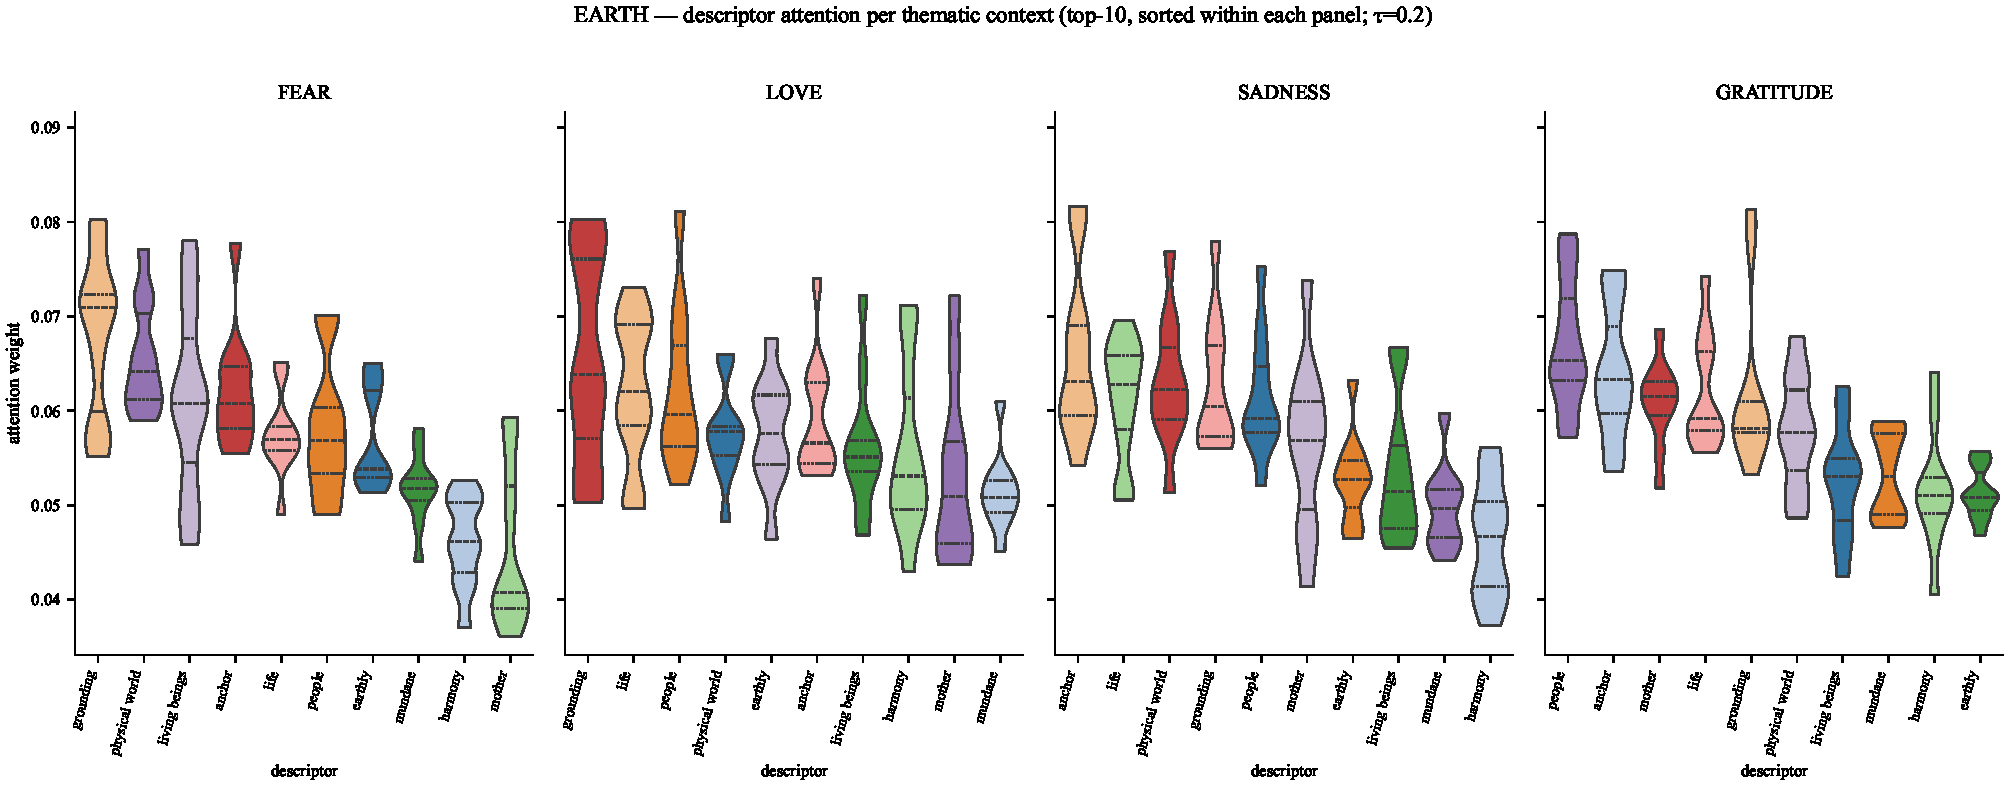
\includegraphics[width=0.9\linewidth]{fig_v1_attention}
    \caption{Contextual similarity distribution for Earth's descriptors across four emotional themes. Each theme comprises ten short sentences written to convey the corresponding emotion (Fear, Love, Sadness, Gratitude), used as contextual probes. Violin plots show, per theme, the distribution of each descriptor's weight over the ten probe sentences, sorted by median weight; higher weights indicate greater cosine similarity of a descriptor to the thematic context. (Weights are a softmax over context--descriptor cosine similarities, a similarity score, not transformer attention.)}
    \label{fig:attention_violin}
\end{figure}

\subsection{Graph-based relational salience}
Beyond the per-descriptor similarity distribution, our framework models the symbolic system as a bipartite symbol--descriptor graph, with additional descriptor--descriptor links where embeddings are highly similar. A Personalized PageRank (PPR) process \citep{lofgren_personalized_2016} can be initialized either from symbol weights or from a free-text context, distributing personalization mass to descriptors by semantic similarity and propagating it through the graph. After convergence, each symbol's PPR score reflects the mass it absorbs via all direct and indirect paths from the context, capturing structural salience from both semantic and topological proximity. We define a symbol's \emph{predicted salience} as the combination of its context-conditioned embedding similarity and this PPR score, so salience is driven partly, but not only, by PageRank: it integrates local semantic fit (similarity) with global network relevance (PPR).

\begin{figure}[tbp]
    \centering
    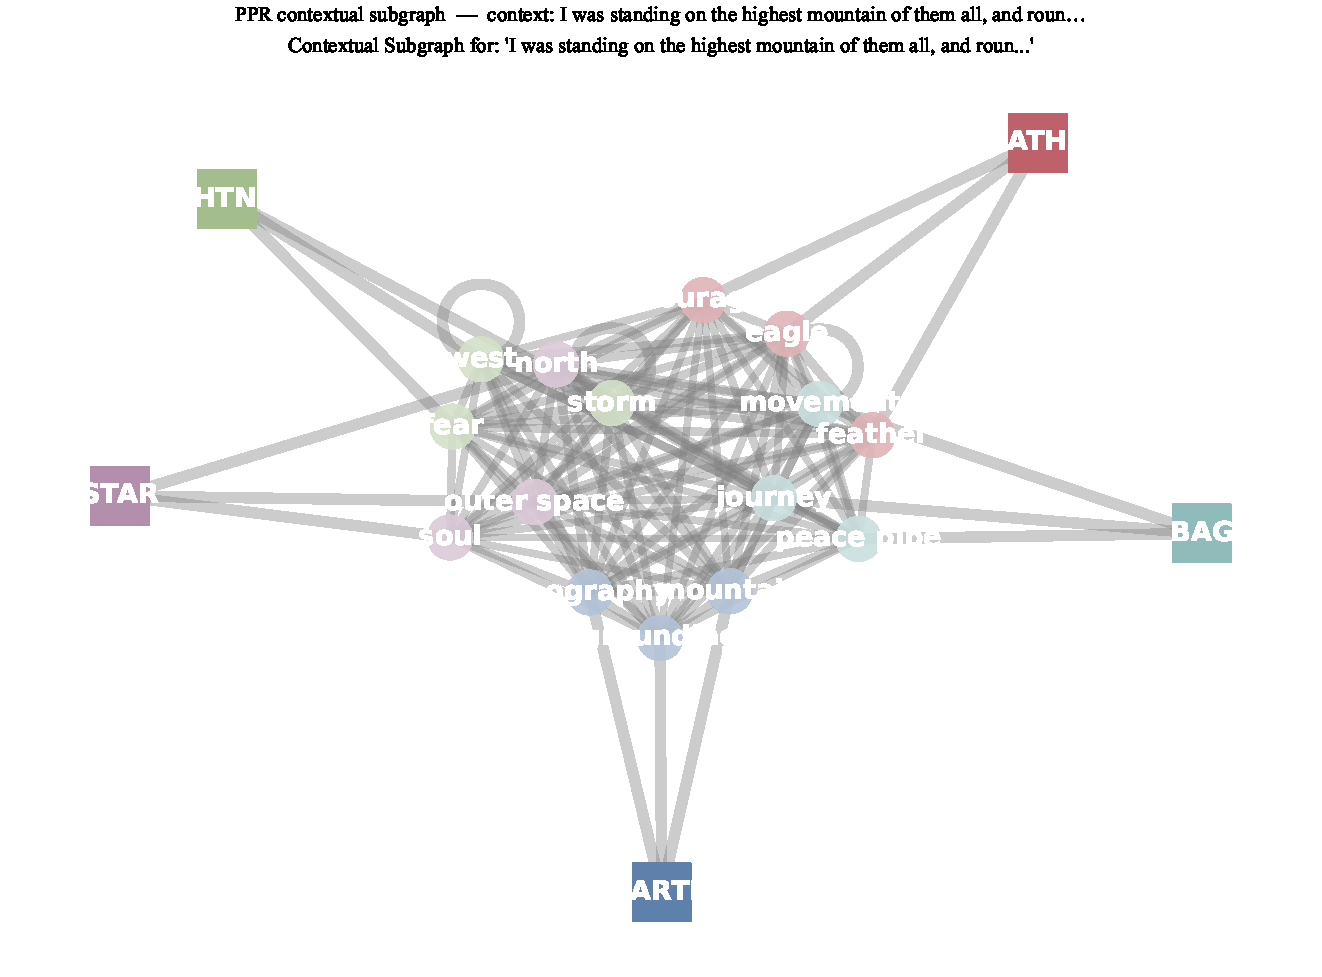
\includegraphics[width=0.7\linewidth]{fig_v1_ppr}
    \caption{Contextual subgraph from Personalized PageRank for a narrative fragment. Symbols (squares) and top descriptors (circles) are colored by symbol, with edge thickness indicating association strength. Baseline centrality is subtracted to highlight relevance emerging specifically from the current context.}
    \label{fig:ppr_subgraph}
\end{figure}

\begin{figure}[tbp]
    \centering
    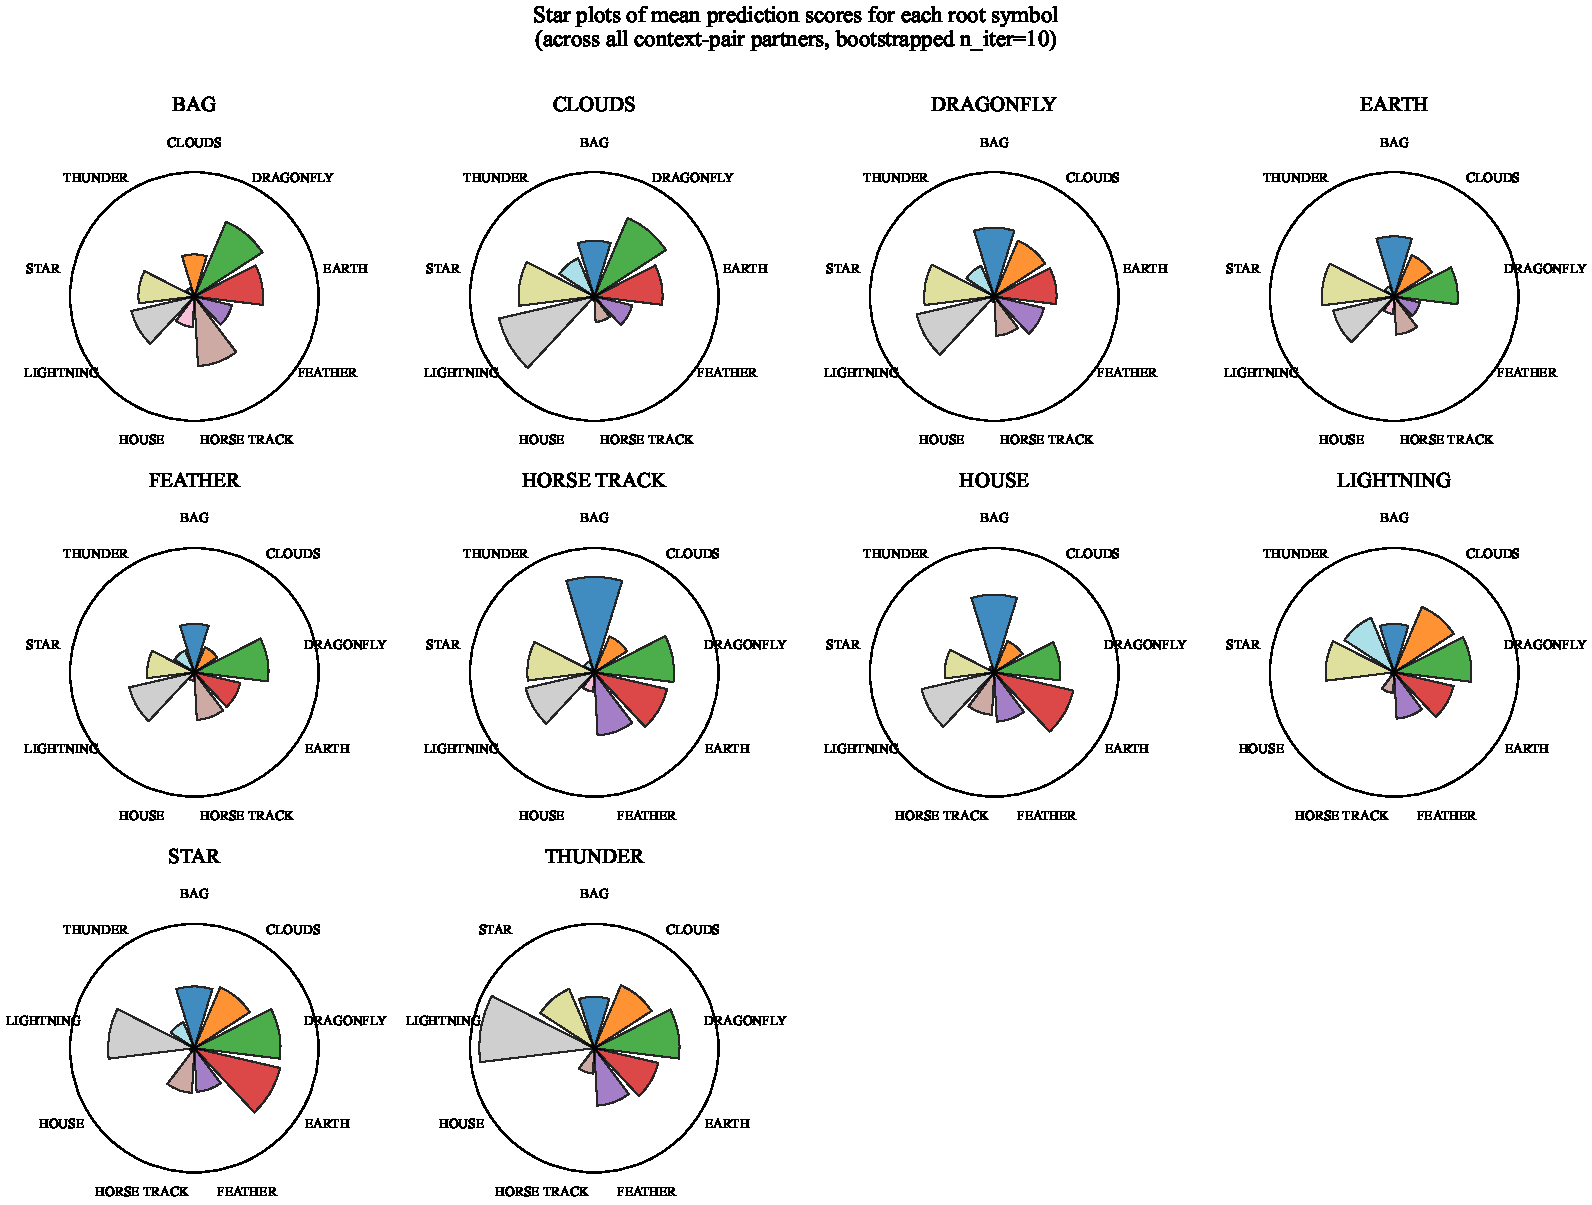
\includegraphics[width=0.9\linewidth]{fig_v1_starplots}
    \caption{Star plots of pairwise contextual salience. For each \emph{root} symbol (one panel), we form a context from the root paired with each other symbol in turn and record the predicted salience (context-conditioned embedding similarity combined with PPR score, \S3.3) of every remaining symbol. Each point on a star is a target symbol; the bar is its mean salience increase over all root+partner pairings, and the radial violin summarizes the distribution of that increase across pairings (bootstrapped over randomly assigned partner weights, $n=20$). Long bars mark targets that the root reliably makes salient regardless of partner; wide violins mark targets whose salience depends strongly on which partner is present.}
    \label{fig:starplots}
\end{figure}

The contextual subgraph (Figure~\ref{fig:ppr_subgraph}) offers an interpretable view of how a given input ``sees'' the symbolic network, surfacing latent thematic clusters and intermediary concepts that would be obscured in the full graph. Figure~\ref{fig:starplots} complements this with a topology-level view of the same salience score. The procedure is: fix a \emph{root} symbol; for every other symbol, build a two-symbol context (root $+$ partner) and compute each remaining symbol's predicted salience as defined above (embedding similarity combined with PPR); then, for each target symbol, average its salience increase across all partners and bootstrap the spread ($n=20$ random partner-weightings). The resulting bar-and-violin star summarizes, per root, which targets it stably co-activates (long bar, narrow violin) versus which depend on the specific partner (wide violin), exposing stable semantic neighbors and highly context-sensitive relationships that embedding similarity alone would not separate.

Together, these analyses establish the \emph{point-level} picture: context redistributes salience across descriptors and symbols. This is real and useful, but it operates on individual nodes. A relational epistemology asks for more: how context reshapes the \emph{relations among} descriptors. We turn to that next.

\FloatBarrier
\section{Quantifying Contextual Distortion of Latent Semantics}
\label{sec:delta}
The similarity-distribution and PPR views above answer \emph{which} descriptors a context foregrounds. They do not directly measure how a context reshapes the geometry that holds the field together: the pattern of pairwise similarities among descriptors. If meaning lives in relations, this geometry is the object of interest, and a context's effect on it is the quantity to measure. We make that quantity explicit.

\subsection{The $\Delta$ coupling matrix}
A context-shift operator $S$ maps the descriptor matrix $D$ to a context-shifted matrix $D' = S(D, c, \theta)$. Throughout we use a gated additive operator,
\begin{equation}
D' = \mathrm{normalize}\!\left( D + \beta \, g_\tau\!\big(\langle D, c\rangle\big) \, c \right),
\end{equation}
which nudges each descriptor toward the context $c$ in proportion to a gated relevance $g_\tau(\langle d_i, c\rangle)$ (defaults $\beta=1.2$, $\tau=0.3$, with per-symbol softmax gating); other strategies (re-embedding in a context-templated prompt, pooled blends, convex hybrids) fit the same slot. The latent geometry of the field at rest is the Gram matrix $C_0 = D D^\top$ of pairwise inner products; under context it becomes $C_1 = D' D'^\top$. The \textbf{$\Delta$ coupling matrix} is their signed difference,
\begin{equation}
\Delta = D' D'^\top - D D^\top, \qquad \Delta_{ij} = \text{change in coupling between descriptors } i \text{ and } j,
\end{equation}
with the diagonal zeroed. $\Delta$ is a direct, per-relation measurement of how context \emph{distorts the latent semantic geometry}: positive entries mark descriptor pairs that context pulls together, negative entries pairs it pushes apart. Rendered as a signed graph over the strongest $|\Delta_{ij}|$ edges, or aggregated to a between-symbol drift map, it localizes contextualization to specific lexical relations rather than to point displacement.

\begin{figure}[tbp]
    \centering
    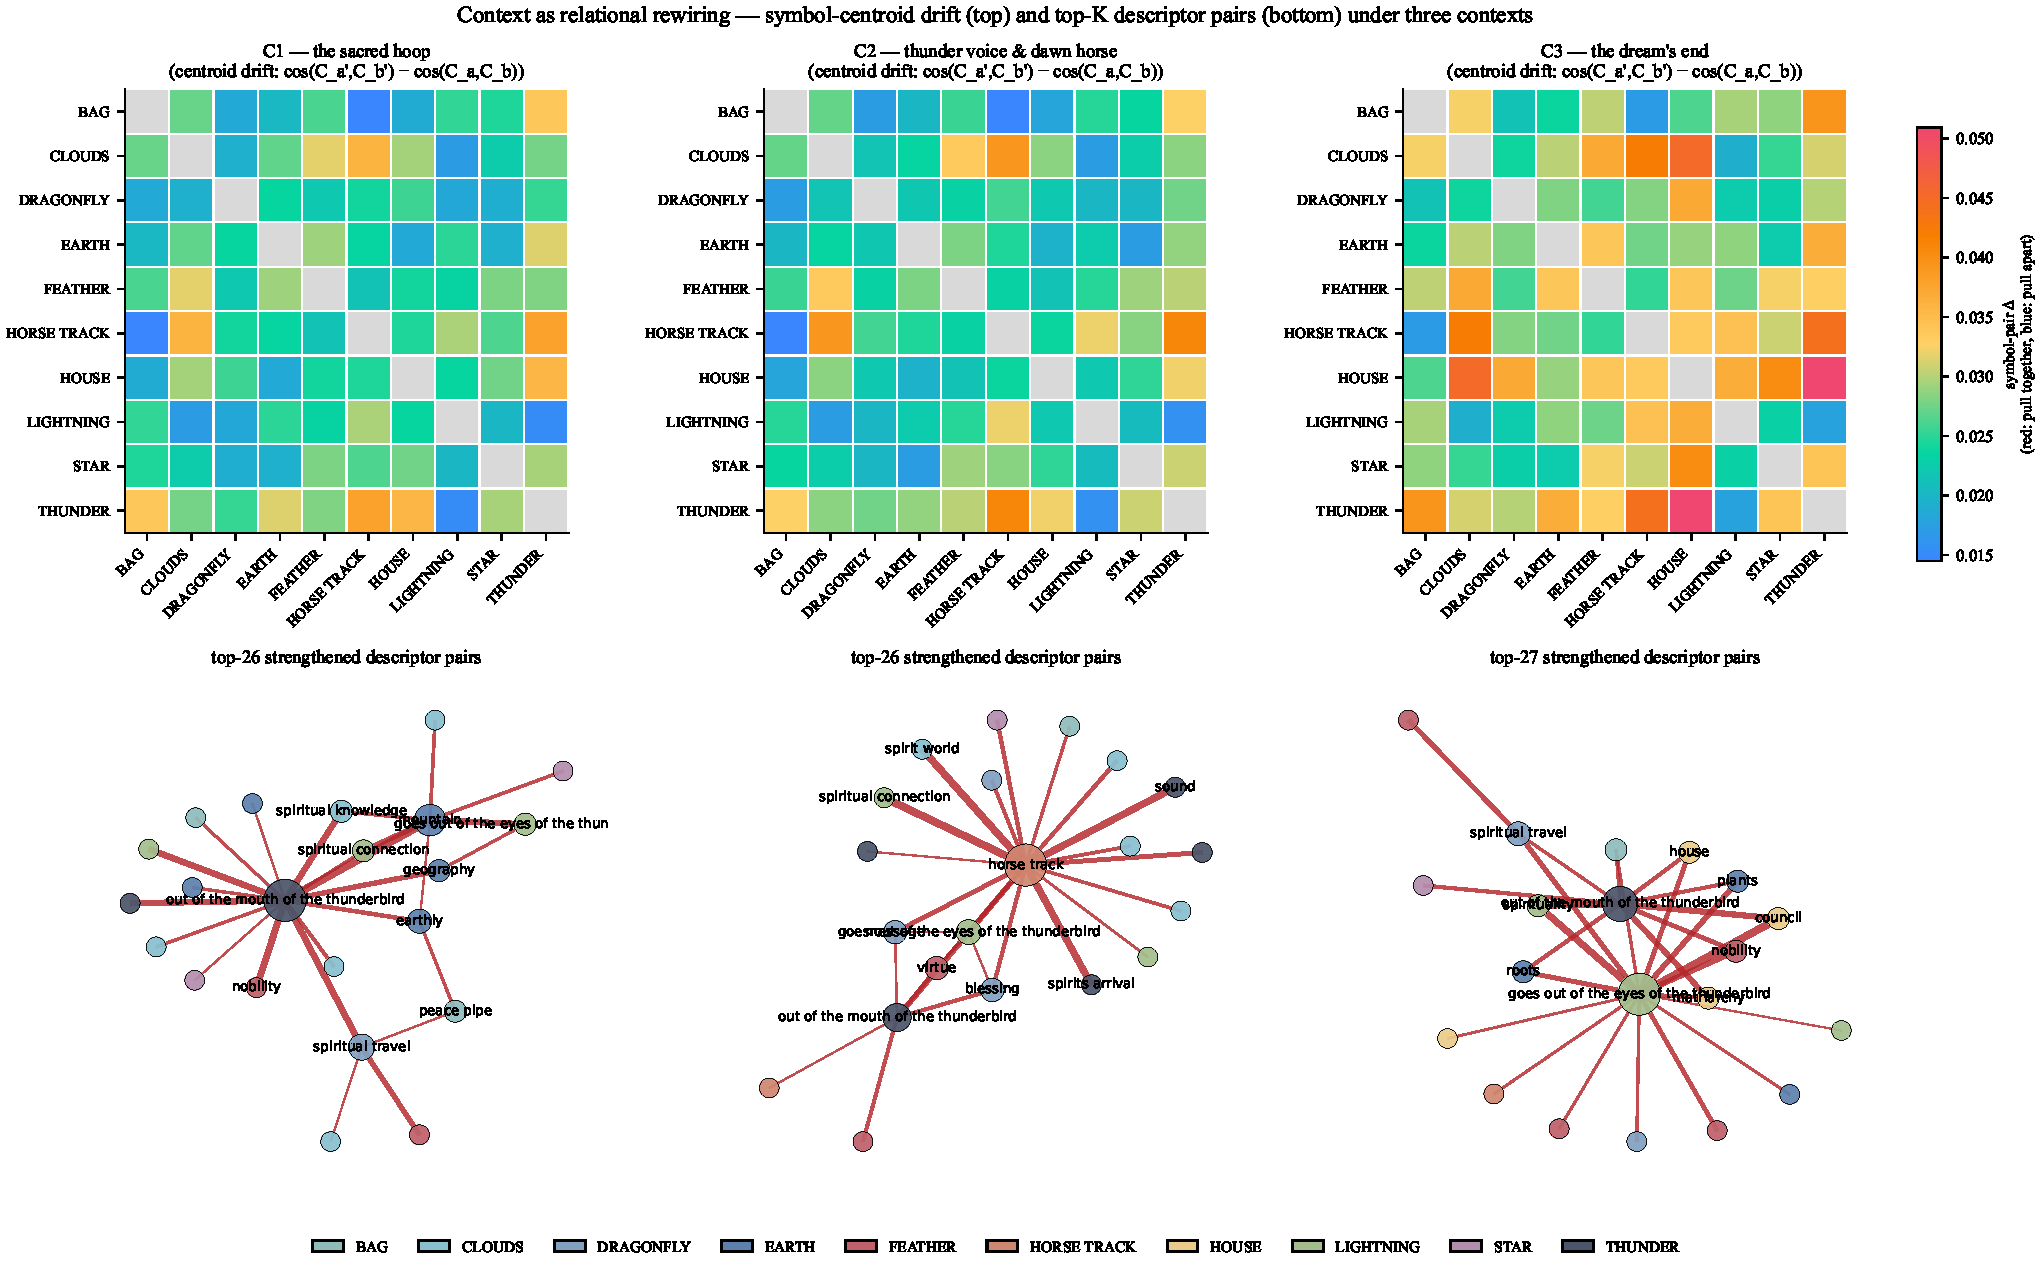
\includegraphics[width=0.95\linewidth]{fig01_delta_graph}
    \caption{Context as relational rewiring. \emph{Top:} between-symbol centroid-drift maps for three narrative contexts $C_1$/$C_2$/$C_3$ over the full Shape Kit ($\cos(C'_a,C'_b)-\cos(C_a,C_b)$; warm = symbols pull together, cool = pull apart). \emph{Bottom:} the corresponding $\Delta$-graphs of the top strengthening descriptor pairs (raw $\Delta$, no centering). The same lexicon yields markedly different relational structures under different framings: their strongest edges are near-disjoint across contexts (top-30 overlap $2$--$9\%$), with edges clustering intra-symbol under one context and bridging symbols under another. Context does not move the symbols; it activates particular relations among their descriptors.}
    \label{fig:delta_graph}
\end{figure}

Figure~\ref{fig:delta_graph} shows three contexts producing three distinct distortion patterns over the same field. This is the Shape Kit's interpretive openness made computationally visible: a single curated lexicon supports many relational configurations, selected by narrative framing.

\textbf{Absolute vs.\ context-specific readings.} Figure~\ref{fig:delta_graph} plots the \emph{raw} $\Delta$ per context, with no centering, and is valid as such. The full fingerprints of $C_1,C_2,C_3$ are nearly collinear as vectors (pairwise cosine $\approx 0.99$): every context strengthens a large, roughly common baseline of relations. But selecting each context's \emph{strongest} edges discards that flat baseline and keeps its context-specific peaks, so the top edges are almost disjoint across contexts (top-30 overlap $2$--$9\%$). The three subgraphs are thus genuinely different structures and already surface most of each context's signature: top-edge selection acts as an implicit de-biasing. Its one blind spot is contamination by generically responsive symbols: $C_1$'s raw graph is Thunder-heavy, though Thunder fires for almost any context, and only subtracting the cross-context mean reveals $C_1$'s \emph{specific} signature, Earth--Star (for $C_2$ and $C_3$, whose distinctive symbols are quieter, the raw subgraph and the centered signature nearly coincide).

The explicit centering used in \S4.3--4.5 (and the per-symbol $z$-scoring for symbol responses) therefore serves a different need than Figure~\ref{fig:delta_graph}. The figure compares contexts \emph{qualitatively}, by reading their subgraphs side by side, a comparison the raw top edges support well, since selection already removes the baseline. Turning $\Delta$ into a \emph{numerical} context-to-context similarity, so that a whole corpus can be clustered or searched automatically (\S4.5), is a different operation: it sums over the \emph{entire} fingerprint, where the $99\%$-collinear baseline dominates and must be removed first. In short, raw $\Delta$ answers ``which relations does this context strengthen most?'' and supports reading a context or comparing a few by eye; centered $\Delta$ answers ``which relations does it strengthen \emph{more than contexts do in general}?'' and is what enables automatic comparison across many contexts.

\subsection{What the readout is, and is not}
We are deliberately precise about the status of $\Delta$, because the honest characterization is also the strongest one. The distortion $\Delta$ measures is, to high accuracy, a \emph{first-order} function of three per-pair quantities: each descriptor's context relevance $s_i = \langle d_i, c\rangle$ and $s_j$, and the descriptors' resting coupling $C_{0,ij}$. Concretely, expanding the gated operator gives $\langle d'_i, d'_j\rangle \propto C_{0,ij} + \beta(g_j s_i + g_i s_j) + \beta^2 g_i g_j$ before renormalization, so a pair strengthens chiefly when both descriptors are context-relevant, modulated by how similar they already were. Empirically, a model in $s_i \cdot s_j$ alone explains only a fraction of $\Delta$ (R$^2 \approx 0.1$--$0.5$), but a model adding $C_{0,ij}$ and its interactions reconstructs the gated-operator $\Delta$ almost completely (R$^2 \approx 0.99$). In other words, $\Delta$ does not recover relational structure that is inaccessible to the encoder: no irreducible whole-graph term is needed; it \emph{re-expresses the encoder's own contextualization in the interpretable coordinate system of a community-curated symbolic field}. This is precisely why it is trustworthy as an interpretability instrument: it is a faithful, legible readout of how the encoder distorts the field, not a higher-order signal whose provenance would be hard to audit. The contribution is the readout (grounded, per-relation, and tied to a designed lexicon), not a claim to compute something a per-descriptor similarity score cannot. (Embedding anisotropy \citep{ethayarajh_contextual_2019} makes the descriptor--context similarities sit in a narrow cone, which is part of why a low-order model suffices.) We exploit this faithfulness in three demonstrations that view the \emph{same} distortion from three angles: in \emph{motion}, as a narrative's trajectory through coupling space (\S4.3); in \emph{confidence}, as the decisiveness with which a context selects a symbol (\S4.4); and in \emph{comparison}, as a similarity between contexts (\S4.5). Section~\ref{sec:discussion} then draws them together.

\subsection{Reading a narrative as a trajectory through coupling space}
Because $\Delta$ is defined per context, a narrative read step by step traces a \emph{path} through coupling space. Figure~\ref{fig:narrative} feeds a twelve-step generic story (a day on the plains; plain English, written for this figure) to a readout calibrated once on a fixed reference battery of oblique probes, and tracks three views: a symbol timeline (the de-biased per-symbol response, whose hot spot migrates with the arc: open grass and horses, a building storm, the strike, shelter, the night sky), the story as a connected trajectory in the principal plane of the residual distortions, and the symbol--symbol couplings with the largest range over the story. Meaning does not sit still as a story unfolds; the distortion readout makes its movement legible.

\begin{figure}[tbp]
    \centering
    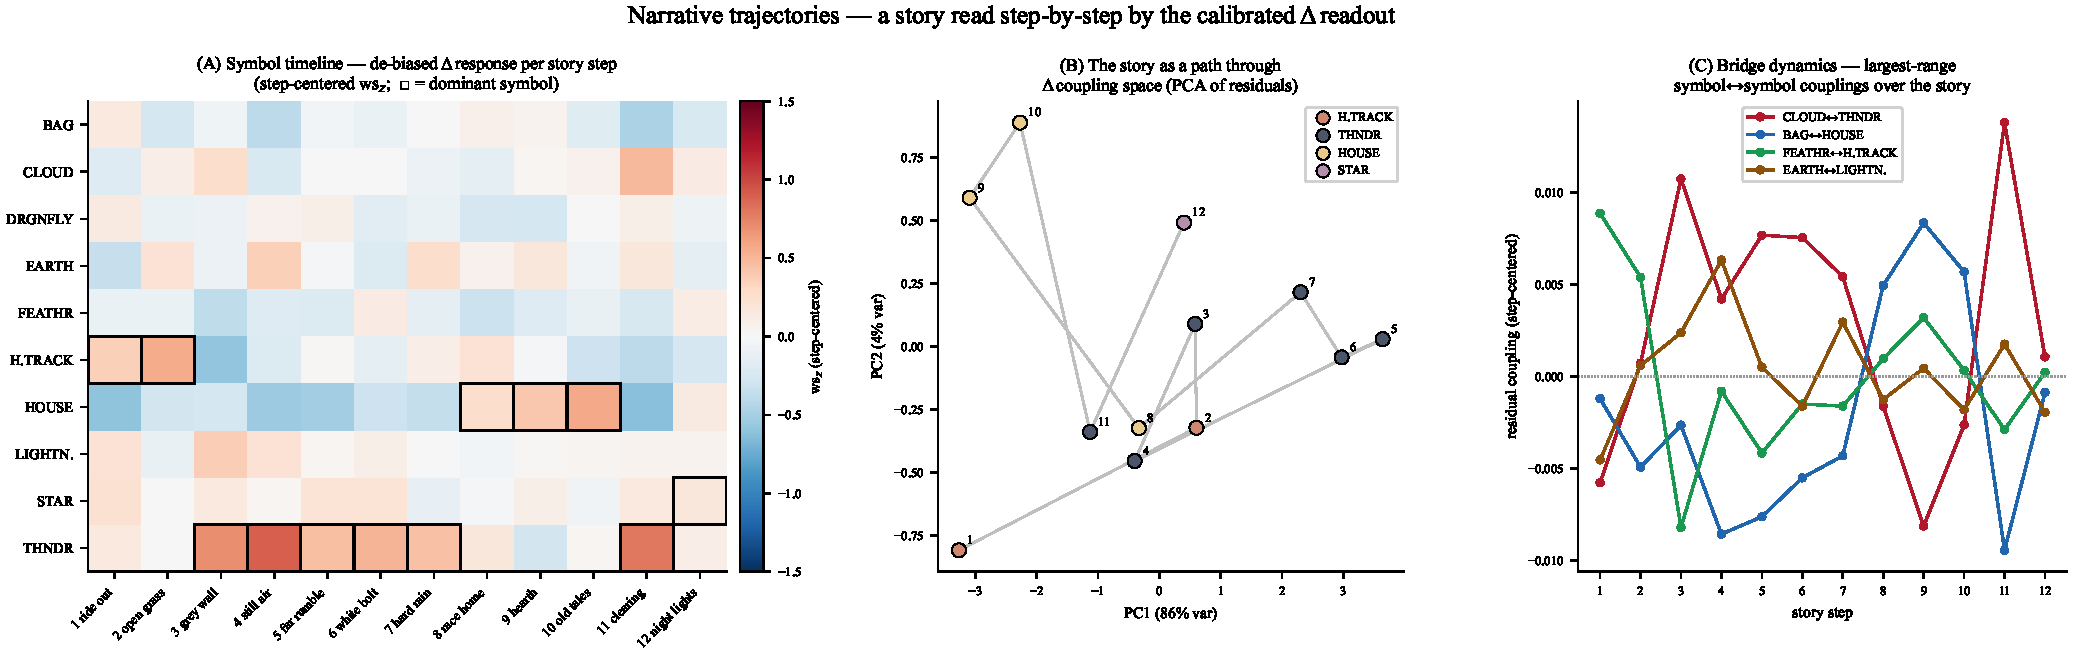
\includegraphics[width=\linewidth]{fig_delta_narrative}
    \caption{Narrative trajectories. A twelve-step story read by the calibrated $\Delta$ readout. \emph{(A)} symbol timeline: de-biased per-symbol response per step, the dominant symbol boxed, the hot spot following the arc. \emph{(B)} the story as a connected path through coupling space (PCA of per-step residual distortions). \emph{(C)} dynamics of the four highest-range symbol--symbol couplings. The story is a trajectory, not a point.}
    \label{fig:narrative}
\end{figure}

\subsection{Distortion margin as an intrinsic uncertainty signal}
The trajectory view tracks \emph{where} the distortion points at each step; we now ask \emph{how decisively} it points there. The same de-biased per-symbol response that drives the timeline in Figure~\ref{fig:narrative} has a top-1 and a top-2 at any given context, and their \emph{margin} measures how sharply the context selects a single symbol over its nearest competitor. Figure~\ref{fig:ambiguity} shows, on a battery of oblique probes, that this margin separates the readout's own correct from incorrect symbol assignments (AUC $\approx 0.78$), and that phrases written to be deliberately ambiguous (constructed so that two symbols fit equally) land in the same low-margin region as the misses. The signal is actionable: ranking probes by margin and abstaining on the least confident raises top-1 accuracy from $67\%$ at full coverage to $\sim\!90\%$ on the most confident third. The readout knows when the context underdetermines the field. (We note honestly that a stricter minimal-pair test, ambiguous phrase versus two disambiguated rewrites of the same scene, did not separate reliably; the readout's resolution is coarser than minimal pairs, and the claim is made at the population level shown.)

\begin{figure}[tbp]
    \centering
    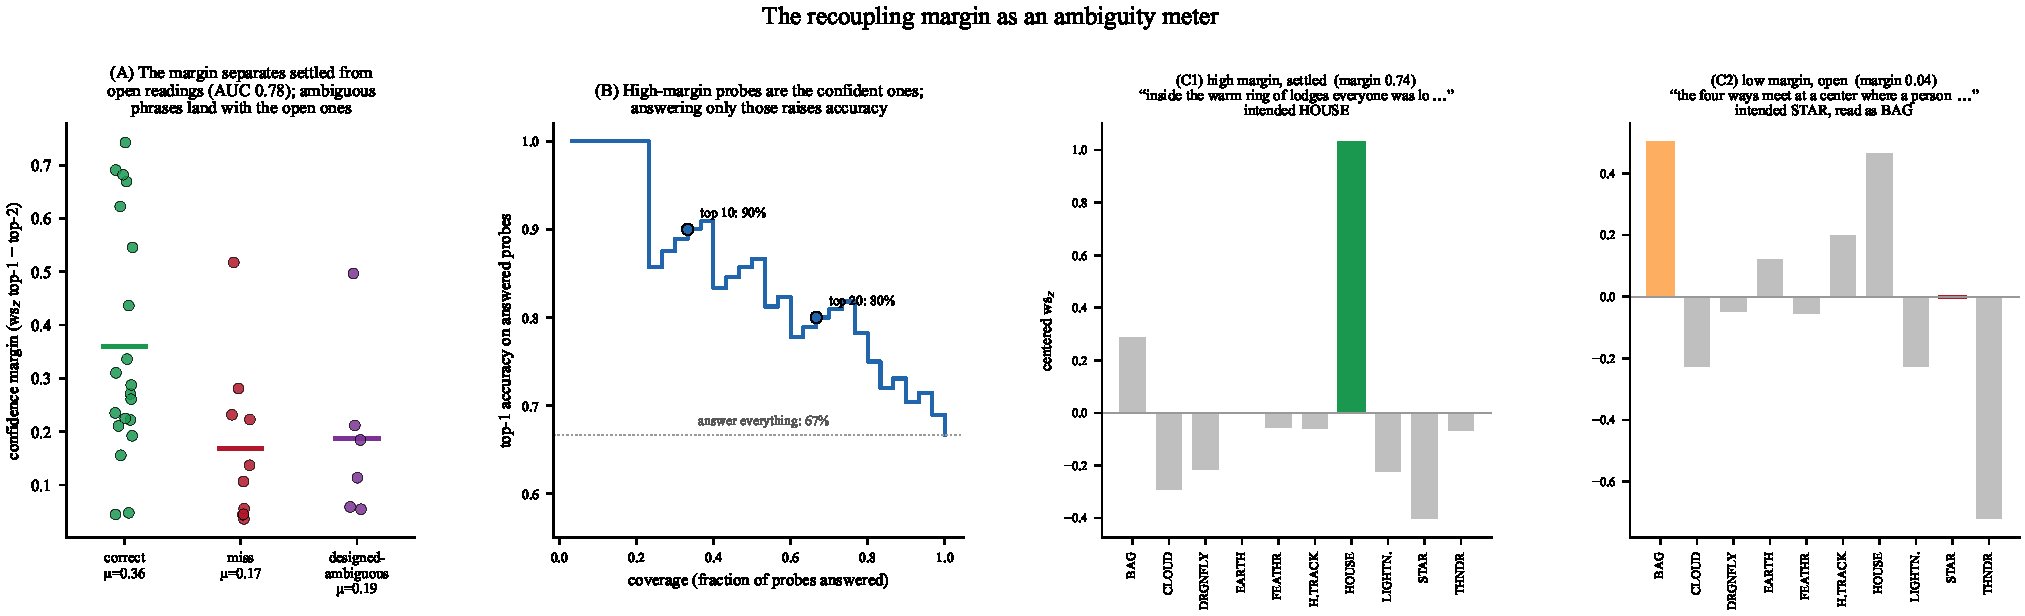
\includegraphics[width=\linewidth]{fig_delta_ambiguity}
    \caption{The readout knows when it doesn't know. \emph{(A)} the confidence margin (top-1 minus top-2 de-biased response) separates the readout's hits from its misses (AUC $0.78$); designed-ambiguous phrases land with the misses. \emph{(B)} selective answering: abstaining on low-margin probes raises top-1 accuracy from $67\%$ to $\sim\!90\%$. \emph{(C)} exemplar profiles: a peaked, confident reading versus a spread, low-margin one over semantically close symbols.}
    \label{fig:ambiguity}
\end{figure}

\subsection{A numerical context-to-context similarity: the field-specific kernel}
Figure~\ref{fig:delta_graph} let us compare a few contexts \emph{qualitatively}, by reading their subgraphs side by side. We now want a \emph{numerical} similarity between contexts (a score, computed from their entire $\Delta$ fingerprints, for how alike any two contexts are) so that a whole corpus can be arranged into a similarity matrix and clustered or searched automatically: two contexts are alike if they distort the field the same way. Because this score sums over the full fingerprint rather than a handful of top edges, it requires one precaution that the subgraph reading did not, and surfacing that precaution is part of the method.

Taken in its raw form, the kernel is dominated by a single mode, about $82\%$ of the variance (Figure~\ref{fig:kernel}A), that captures not \emph{how} a context reshapes the field but merely \emph{how strongly} it engages the descriptor bank at all (correlation $0.84$ with a pure activation-strength predictor). Overall activation strength is a generic property of a context, not a fact about the Lakota field; this is exactly why the raw kernel barely changes when we read the same contexts through an unrelated lexicon (a generic emotion set; $r=0.93$). In other words, before correction the kernel is measuring context ``loudness,'' not the structure of the symbolic system: a limitation, not a virtue.

A single standard, label-free operation removes it: subtracting the top principal component of the battery residuals (``all-but-the-top'' \citep{mu_allbutthetop_2018}). After this step the loudness mode is gone (its correlation with activation strength falls $0.84 \to -0.13$) and the kernel becomes \emph{field-specific and content-bearing}. It now depends on the chosen lexicon (cross-lexicon agreement drops $0.93 \to 0.76$, meaning the similarity finally reflects the Lakota structure rather than a generic magnitude); it aligns with sentence meaning (agreement with sentence-embedding similarity rises $0.31 \to 0.69$), and hierarchical clustering recovers coherent thematic registers readable directly off the probe sentences (storm and numinous sky; honor and deeds; caretaking; growth and soil; Figure~\ref{fig:kernel}B).

Two points connect this back to the rest of the paper. First, this is the \emph{same} centering already built into the per-symbol readouts of \S4.1--4.4, so those views were never affected by the loudness mode; the kernel simply makes the mode visible and shows why removing it is necessary whenever $\Delta$ is used to compare contexts. Second, we state the scope plainly: the cleaned kernel is an \emph{interpretable, field-specific} readout of how contexts distort the lexicon, not a general-purpose similarity metric: it does not separate same-target contexts better than raw sentence embeddings do. Its distinctive value is that, unlike a raw embedding kernel, its groupings are legible in the categories of the curated field itself.

\begin{figure}[tbp]
    \centering
    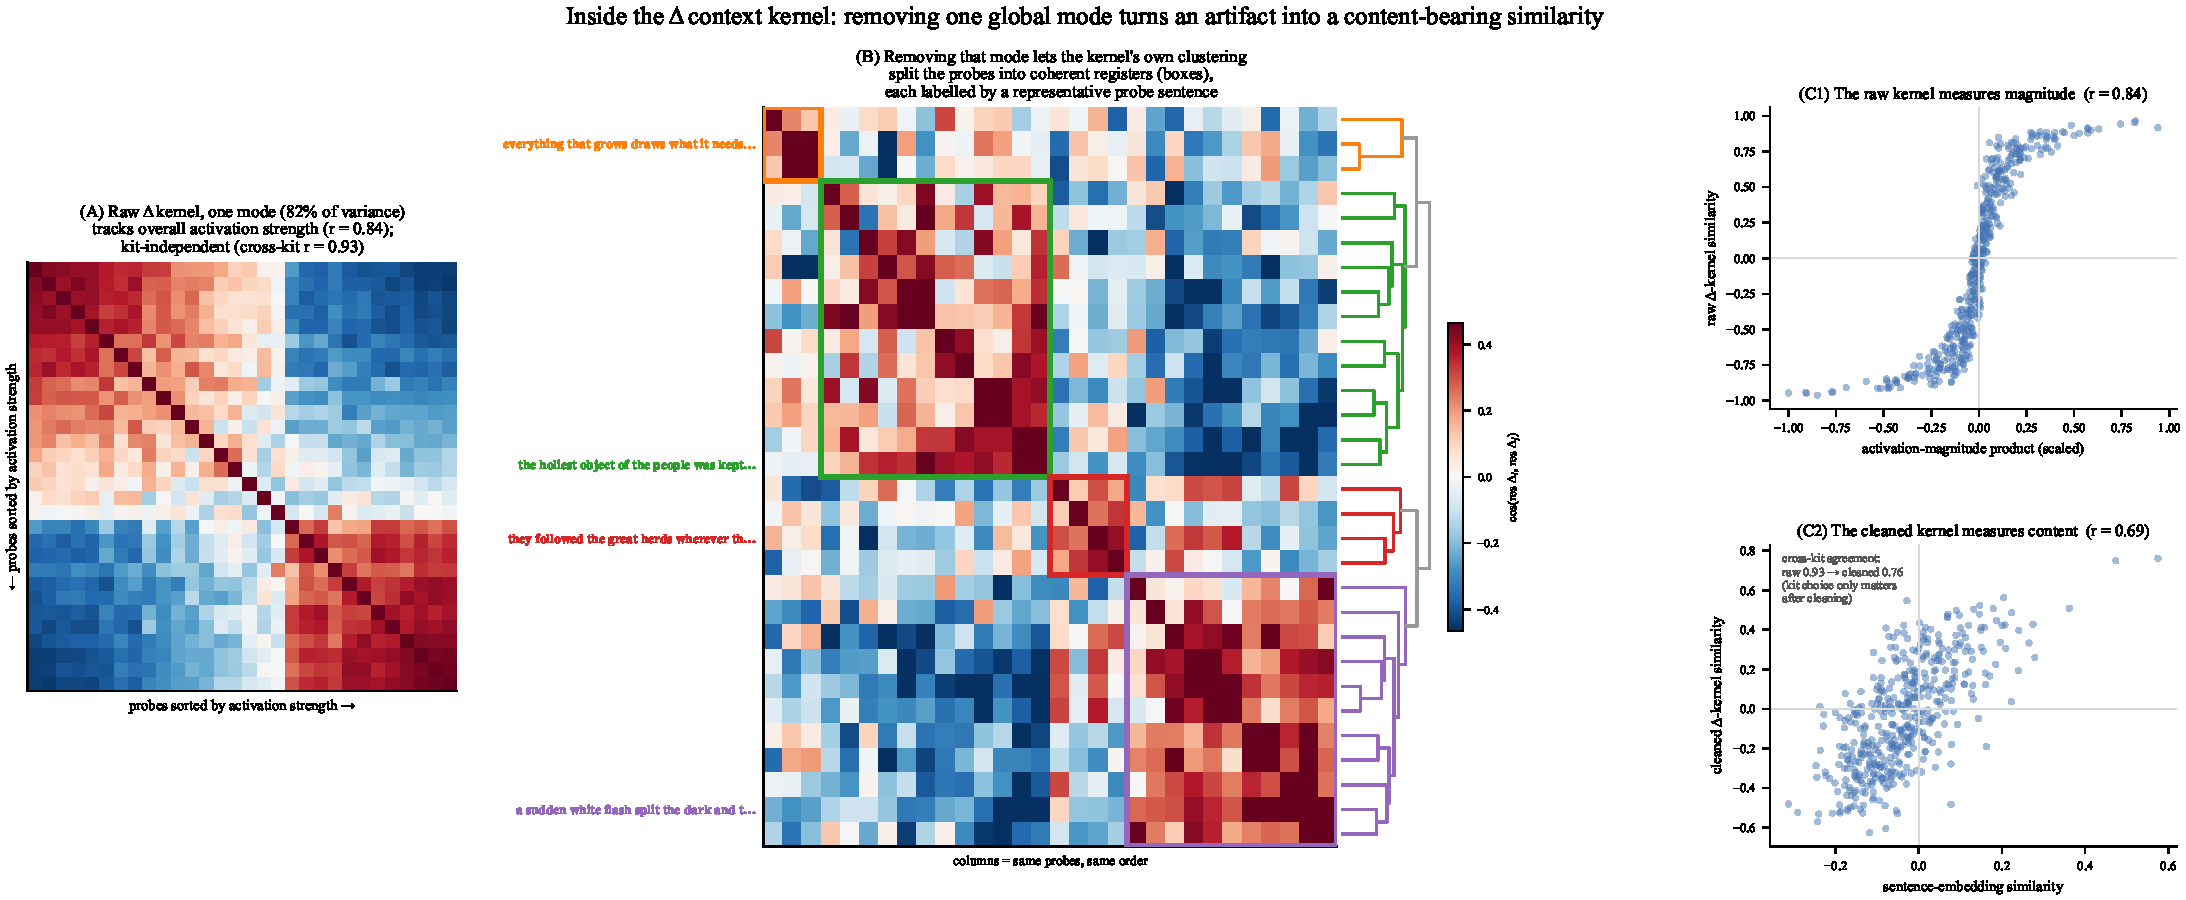
\includegraphics[width=\linewidth]{fig_delta_kernel}
    \caption{Inside the $\Delta$ context kernel. \emph{(A)} the raw kernel, probes sorted by activation strength: one mode ($82\%$ of variance) tracks overall activation magnitude ($r=0.84$) and is lexicon-independent (cross-kit $r=0.93$). \emph{(B)} after removing that single mode, coherent thematic registers emerge, with rows labeled by the probe sentences themselves and ordered by the kernel's own clustering, with no category labels used. \emph{(C)} the raw kernel measures magnitude; the cleaned kernel measures content (agreement with embedding similarity $0.31\to0.69$).}
    \label{fig:kernel}
\end{figure}

\subsection{Robustness: is it signal, and is it encoder-specific?}
\label{sec:robust}
A natural question is whether these distortions \emph{matter}: whether they are structured signal rather than an inevitable consequence of moving the descriptors at all, and whether they are an artifact of one encoder. Two compute-only checks address both (Figure~\ref{fig:robustness}).

\textbf{Null model.} For each oblique probe we replace its real context-shift with a \emph{random} shift of equal magnitude ($\|D'-D\|_F$ matched to within $4\%$) and ask whether the de-biased readout still recovers the intended symbol. It does not: real contexts ground at $67\%$ top-1 / $93\%$ top-3, while magnitude-matched random shifts collapse to $8\%$ / $31\%$, essentially the $10\%$ / $30\%$ chance rates. The measured distortions are therefore structured signal tied to a context's meaning, not a by-product of the shift's size.

\textbf{Multi-embedder.} Re-running the grounding battery on three unrelated encoders (Qwen3-0.6B, $1024$-d; MPNet, $768$-d \citep{song_mpnet_2020}; and MiniLM, $384$-d \citep{wang_minilm_2020}), grounding holds throughout (top-1 $67\%$, $70\%$, $57\%$; all far above chance), and the three encoders assign the same symbol to a probe $73\%$ of the time. Accuracy tracks encoder capacity (the smallest model, MiniLM, is weakest, as expected), but the readout reflects the symbolic system and the probe semantics rather than any single model's geometry. These checks answer the ``signal vs.\ noise'' and ``one-model artifact'' objections; validating that the distortions matter \emph{in the way the paper claims} (that the relational patterns resonate with the tradition) is the role of community review (\S\ref{sec:discussion}).

\begin{figure}[tbp]
    \centering
    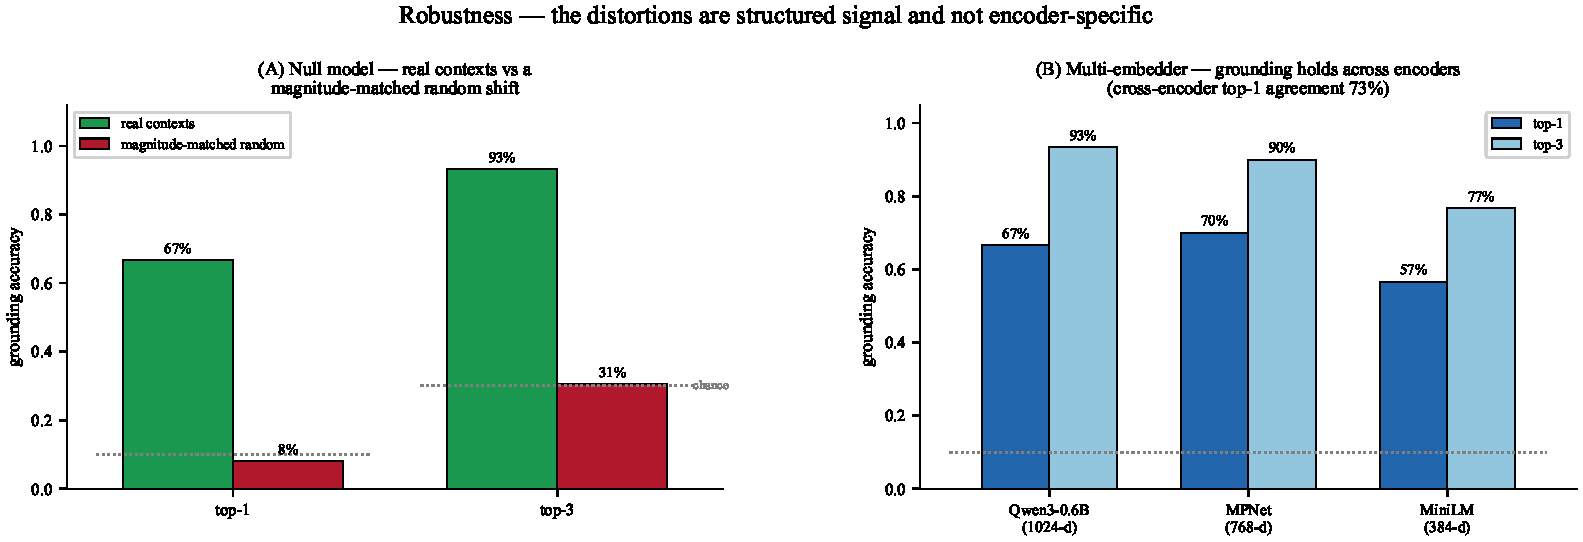
\includegraphics[width=\linewidth]{fig_delta_robustness}
    \caption{Robustness. \emph{(A)} Null model: real contexts recover the intended symbol far above a magnitude-matched random shift (top-1 $67\%$ vs $8\%$; top-3 $93\%$ vs $31\%$; chance $10$/$30\%$), so the distortions are structured signal, not a by-product of shift magnitude. \emph{(B)} Multi-embedder: grounding holds across three unrelated encoders (Qwen3, MPNet, MiniLM), with $73\%$ cross-encoder agreement on the assigned symbol: the readout is not an artifact of one model's geometry.}
    \label{fig:robustness}
\end{figure}

\FloatBarrier
\section{Probing Symbolic Ambiguity Across Modalities}
\label{sec:multimodal}
The $\Delta$ readout depends only on a context \emph{vector} in the descriptor space; nothing about it is specific to text. Any encoder that lands an input in that space can drive it, so the ambiguity of a curated symbolic field can be probed not only through written context but through other modalities, fitting for a tradition carried by story, song, and sound as much as by writing. We demonstrate this with audio, treating sound as a first-class probe of the field rather than a downstream add-on.

We are explicit about the mechanics. A contrastive audio encoder (CLAP \citep{wu_clap_2023}) shares an audio--text space, but its \emph{text} tower is too weak to represent the curated descriptors directly: it grounds the oblique probes of \S4 only at chance. We therefore use a \emph{bridge}: a recording is embedded with CLAP, scored against a generic vocabulary of acoustic scenes (``thunder,'' ``crackling fire,'' ``ocean waves,'' \ldots), and the resulting blend of labels becomes a text context for the readout. CLAP recognizes real field recordings cleanly (birdsong $0.96$, thunder $0.96$), so the bridge is reliable for natural sound even where the direct audio--descriptor route is not.

Driven by sound, the readout produces structured, well-separated, interpretable signatures (Figure~\ref{fig:soundscape}A): each sound family activates a distinct \emph{subnetwork} of symbol couplings (storm$\to$Thunder/Lightning, hearth$\to$Feather/House, water$\to$Earth/Clouds), overwhelmingly between symbols (top edges $82$--$98\%$ cross-symbol) and mutually near-orthogonal across families. Every sound strengthens couplings across the field (the context pulls all descriptors toward it, $\Delta>0$ throughout at near-uniform magnitude); the subnetworks are the family-specific \emph{residual} on that shared mode: differential emphasis, never a weakening. The ambiguity connection is direct: a sound need not name a symbol to surface its meaning, and a sound that sits between registers surfaces a \emph{blend} of symbols (ambiguity made audible), just as oblique text did in \S4. \emph{Morphing} between two recordings (Figure~\ref{fig:soundscape}B) traverses the field continuously, the storm register fading as the hearth register rising, so the ambiguous in-between is itself navigable. Sound is thus a second, independent window onto the same computational account of symbolic ambiguity, not merely a different input format. (The bridge is a measured, honest claim: it routes audio through acoustic labels, not a fused audio--symbol space; a stronger shared encoder would remove the intermediate step.)

\begin{figure}[tbp]
    \centering
    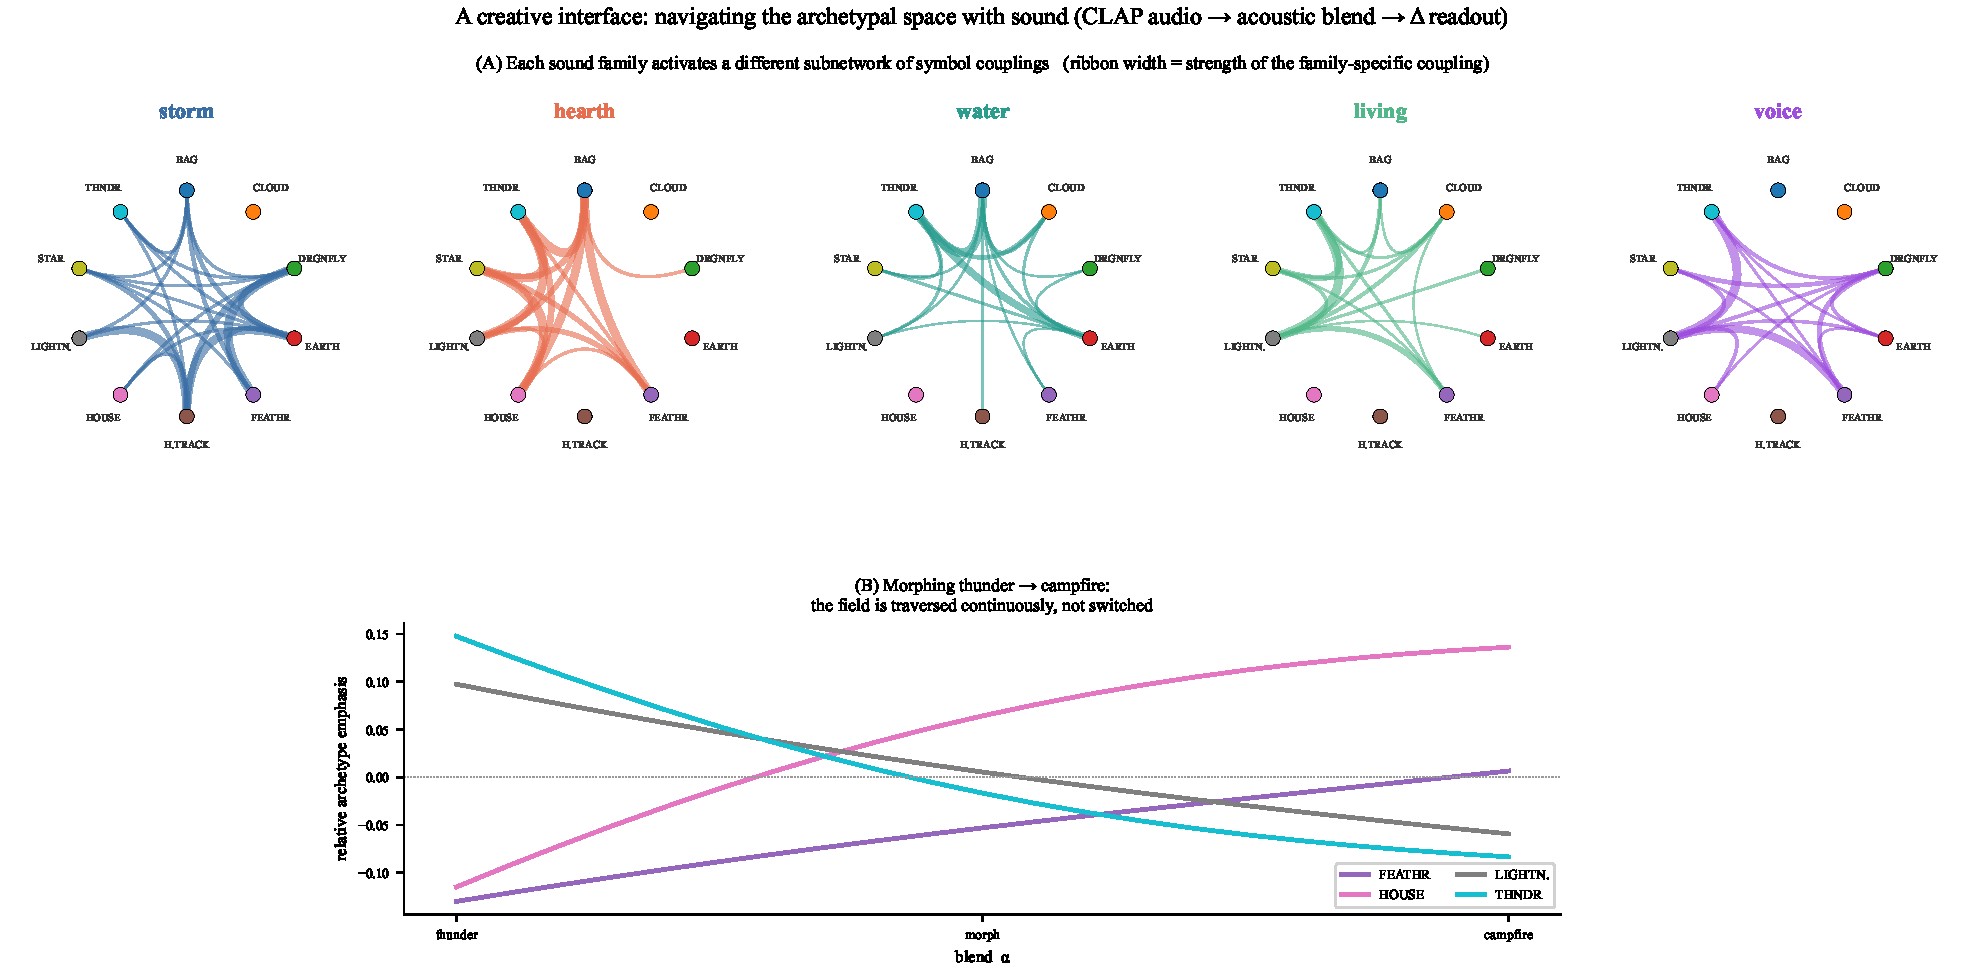
\includegraphics[width=\linewidth]{fig_delta_soundscape}
    \caption{Navigating the archetypal space with sound. CC/PD field recordings (Wikimedia Commons) drive the readout through an audio$\to$acoustic-label$\to$text bridge. \emph{(A)} one chord diagram per sound family: ribbons are the symbol couplings that family distinctively activates (width = magnitude of the family-specific coupling, aggregated over its top descriptor-pair edges). Each family lights up a different subnetwork (storm couples Thunder/Lightning, hearth Feather/House, water Earth/Clouds), and the couplings are overwhelmingly \emph{between} symbols (top edges $82$--$98\%$ cross-symbol). Every sound strengthens couplings ($\Delta>0$ throughout); ribbons show each family's coupling \emph{relative to the average sound}, i.e.\ differential emphasis, not weakening. \emph{(B)} morphing thunder\,$\to$\,campfire: the storm symbols (Thunder, Lightning) yield to the hearth symbols (House, Feather) continuously across the blend: the field is traversed, not switched. (Audio licenses to be verified per file before publication.)}
    \label{fig:soundscape}
\end{figure}

\FloatBarrier
\section{Discussion}
\label{sec:discussion}
The analytical figures of Section~\ref{sec:delta} are not four methods that might agree or disagree; they are four projections of a single object: the context-induced distortion $\Delta$ of the field's latent geometry. Figure~\ref{fig:delta_graph} shows its \emph{structure} (which relations a single context strengthens or weakens); Figure~\ref{fig:narrative} shows its \emph{motion} (how that structure travels as a narrative unfolds); Figure~\ref{fig:ambiguity} shows its \emph{confidence} (how decisively a context resolves the field); and Figure~\ref{fig:kernel} shows its \emph{comparability} (how the distortions of two different contexts relate). Section~\ref{sec:multimodal} adds a view along a different axis: the same object is \emph{modality-agnostic}, producing structured, separable signatures when driven by sound just as by text. Read this way, the results cannot conflict in the way one might fear when several analyses are stacked together: there is one measured quantity, examined at the level of a single relation, a single context, a sequence of contexts, pairs of contexts, and a non-textual input.

More than merely non-conflicting, the views reinforce one another through a shared calibration. The timeline and the margin read the \emph{same} de-biased per-symbol response; the trajectory and the kernel both operate on the \emph{same} mean-removed residual distortion. The kernel analysis (Figure~\ref{fig:kernel}) is, in effect, an audit of that de-biasing: it shows that the dominant mode of the raw distortion is an activation-magnitude artifact, and that subtracting it is precisely what exposes content. That same subtraction is what keeps the narrative timeline and the confidence margin from being dominated by how ``loud'' each context happens to be. A weakness surfaced in one view is therefore diagnosed and corrected consistently across all of them, which is the main reason we present them together rather than as independent results.

A single honest characterization runs through all four. The distortion is, to high accuracy, a first-order, similarity-driven reshaping of the encoder's own representation (\S4.2); we do not claim it recovers structure the encoder lacks. Its contribution is to make that internal reshaping \emph{legible} (per relation, in the coordinate system of a community-curated field) and, as the demonstrations show, legible enough to support a usable uncertainty signal and a content-bearing context similarity. Where a claim would overreach we mark the boundary: the readout's resolution is coarser than minimal pairs (\S4.4), and the de-biased kernel does not separate same-target contexts better than raw embeddings do (\S4.5). These are limits of the instrument, stated as such.

Two broader limitations bound the present results. First, the robustness checks of \S\ref{sec:robust} establish that the distortions are signal (they beat a magnitude-matched null) and survive across three encoders, but they are computed on a single curated field; disentangling how much structure is intrinsic to \emph{this symbolic system} from what holds for embedding models in general would benefit from additional lexicons and a wider encoder pool. Second, and more fundamentally, the framework reads how a model \emph{represents} a curated field; it does not by itself validate that representation against the living tradition. That validation is the role of community-grounded review (structured interpretation of selected $\Delta$-graphs and signatures with knowledge holders), which the broader project treats as the primary form of evaluation rather than a supplement to it. These limits also mark the work's forward edges: extending the instrument across many curated systems, to ask how each distinctively engages a given text, and inverting it from analysis toward tradition-anchored design (\S Creative Applications), are each substantial enough, methodologically and ethically, to warrant their own treatment beyond this paper.

The through-line returns to where the framework began. If meaning is the position of a thing in a living web of relations, then the quantity to measure under context is the reconfiguration of that web, not the displacement of a point. The $\Delta$ readout makes exactly that reconfiguration legible, and the four views are four ways of attending to it, a formal echo of \emph{Mitákuye Oyás'i\textipa{N}}: meaning read as relation, and change in meaning as change in relation.

\FloatBarrier
\section{Creative Applications}
The same readouts make the framework a generative instrument, and the multimodal probe of \S\ref{sec:multimodal} is the first creative affordance: a \emph{sonic interface to the symbolic field}. A performer or installation can navigate the field by sound in real time and morph between recordings to move through the space \emph{between} readings: a tool for sound-led, improvisatory storytelling that keeps a non-textual tradition non-textual. Three text-side affordances follow from the same machinery. \emph{Associative expansion}: the $\Delta$-graph and contextual subgraph of a narrative fragment surface relational pathways (which couplings a framing strengthens, which symbols it bridges) that a poet, storyteller, or visual artist might not otherwise consider \citep{varshney_associative_2016, gross_lexical_2012, rick_supermind_2023}. \emph{Structural prompting}: rather than retrieving text (as in RAG) or passing raw context, one can condition a generator on the \emph{structural} motifs the readout exposes: top $\Delta$-edges, a descriptor's migration to a new nearest symbol, or a turning point in a narrative trajectory (\S4.3). Generation then stays grounded in the field's own logic rather than free-associating away from it. \emph{Continuous morphing}: interpolating between two contexts (of any modality) yields a trajectory of relational states, a controllable dial between two readings rather than a switch. Finally, because the readout exposes \emph{where} a context is ambiguous (\S4.4), ambiguity becomes a creative dial in its own right (high-entropy contexts maximize associative divergence, low-entropy ones keep generation tightly grounded), turning the very property other models flatten into a control surface. Together these let traditional narrative frameworks such as Lakota dream storytelling blend with AI-assisted generation in a way that preserves cultural specificity while fostering novel expression.

These affordances are not ends in themselves but components of a larger aim: \emph{design practice that works with living symbolic traditions rather than extracting from them}. The same instrument that reads how a story rewires a field supports the inverse move: surfacing the symbolic structure that a community's stories activate, combining the structures that several narratives induce, and using the result to inform new design developed in dialogue with knowledge holders. Working across narratives this way is methodologically and ethically substantial: it raises questions of whose stories, under what consent, and who authors and benefits from what is made, questions a methods paper cannot discharge in passing. We therefore treat tradition-anchored design as a dedicated future direction, to be developed as participatory design research under the community-governed commitments stated below (\S Ethical Considerations), and flag it here because it is the affordance the framework most naturally grows toward: a generative, culturally anchored complement to the analytic instrument developed above.

\section{Ethical Considerations}
This project is conducted in active collaboration with Indigenous community partners, with the last author being an Oglala Lakota knowledge holder. All symbolic material and interpretations are developed in accordance with community protocols and with guidance from cultural experts; the descriptor sets and context sentences shown here are chosen for public demonstration, and materials that belong to the community are not disclosed. The work is supported by the Abundant Intelligences program, which fosters AI systems developed in respectful interaction with Indigenous knowledge systems \citep{lewis_indigenous_2020}. Our design, data use, and dissemination follow the CARE Principles for Indigenous Data Governance \citep{carroll_care_2020} and the broader commitments of Indigenous data sovereignty \citep{kukutai_indigenous_2016}, honoring community authority over the knowledge represented here. We stress that descriptor curation by knowledge holders is not a limitation of the method but its precondition: community-grounded AI requires Indigenous expertise to mean anything, and the framework is built so that this expertise governs what the instruments read.

\bibliographystyle{plainnat}
\bibliography{references}

\end{document}
